%\documentclass[handout]{beamer} %Makes Handouts
\usetheme{Singapore} %Gray with fade at top
\useoutertheme[subsection=false]{miniframes} %Supppress subsection in header
\useinnertheme{rectangles} %Itemize/Enumerate boxes
\usecolortheme{seagull} %Color theme
\usecolortheme{rose} %Inner color theme

\definecolor{light-gray}{gray}{0.75}
\definecolor{dark-gray}{gray}{0.55}
\setbeamercolor{item}{fg=light-gray}
\setbeamercolor{enumerate item}{fg=dark-gray}

\setbeamertemplate{navigation symbols}{}
\setbeamertemplate{mini frames}[default]
\setbeamercovered{dynamics}
\setbeamerfont*{title}{size=\Large,series=\bfseries}

%\setbeameroption{notes on second screen} %Dual-Screen Notes
%\setbeameroption{show only notes} %Notes Output

\newcommand{\heading}[1]{\noindent \textbf{#1}\\ \vspace{1em}}

\usepackage{bbding,color,multirow,times,ccaption,tabularx,graphicx,verbatim,booktabs,fixltx2e}
\usepackage{colortbl} %Table overlays
\usepackage[english]{babel}
\usepackage[latin1]{inputenc}
\usepackage[T1]{fontenc}

%\author[]{Thomas J. Leeper}
\institute[]{
  \inst{}%
  Department of Political Science and Government\\Aarhus University
}

\usepackage{tikz}
\usetikzlibrary{shapes,arrows}
\usetikzlibrary{decorations.pathreplacing}

\title{Methods Supplementary Lecture 2:\\Survey Analysis}

\date[]{}

\begin{document}

\frame{\titlepage}

\frame{\tableofcontents}

\section{Linear Regression Analysis}
\frame{\tableofcontents[currentsection]}


\frame{
	\frametitle{Uses of Regression}
	\begin{enumerate}\itemsep2em
	\item Description
	\item Prediction
	\item Causal Inference
	\end{enumerate}
}

\frame{
	\frametitle{Descriptive Inference}
	\begin{enumerate}\itemsep1em
	\item We want to understand a \textit{population} of cases
	\item We cannot observe them all, so:
		\begin{enumerate}
    		\item Draw a \textit{representative} sample
    		\item Perform mathematical procedures on sample data
    		\item Use assumptions to make inferences about population
    		\item Express uncertainty about those inferences based on assumptions
		\end{enumerate}
	\end{enumerate}
}

\frame{
	\frametitle{Parameter Estimation}
	\begin{itemize}\itemsep1em
    	\item We want to observe population \textit{parameter} $\theta$
    	\item If we obtain a representative sample of population units:\\
    		\begin{itemize}\itemsep1em
        		\item Our sample statistic $\hat{\theta}$ is an unbiased estimate of $\theta$
        		\item Our sampling procedure dictates how uncertain we are about the value of $\theta$
    		\end{itemize}
	\end{itemize}
}

\frame{
	\frametitle{An Example}
	\begin{itemize}
	\item We want to know $\bar{Y}$ (population mean)
	\item Our \textit{estimator} is the sample mean formula which produces the sample \textit{estimate} $\bar{y}$:
		\begin{equation}
		\bar{y} = \frac{1}{n}\sum_{i=1}^{n}y_i
		\end{equation}
	\item The \textit{sampling variance} is our uncertainty:
	\begin{equation}
	Var(\bar{y}) = \frac{s^2}{n}
	\end{equation}
	where $s^2 = $ sample element variance
	\end{itemize}
}

\frame{
	\frametitle{Uncertainty}
	\begin{itemize}\itemsep1em
		\item We never know $\theta$
		\item Our $\hat{\theta}$ is an estimate that may not equal $\theta$
			\begin{itemize}
    			\item Unbiased due to \textbf{Law of Large Numbers}
    			\item For $\bar{y}$: $N(Y, \sigma^2) $
			\end{itemize}
    	\item The size of sampling variance depends on:
    		\begin{itemize}
        		\item Element variance
        		\item Sample size!
    		\end{itemize}
    	\item Note: $SE(\bar{y}) = \sqrt{Var(\bar{y})}$
    	\item We may want to know $\hat{\theta}$ per se, but we are mostly interested in it as an estimate of $\theta$
	\end{itemize}
}

\frame{
	\frametitle{Causal Inference}
	\begin{enumerate}\itemsep1em
	\item<2-> Everything that goes into descriptive inference
	\item<3-> Plus, philosophical assumptions
	\item<4-> Plus, randomization \textit{or} perfectly specified model
	\end{enumerate}
}


\frame{\frametitle{Questions about philosophical assumptions?}}

\frame<1-5,2>[label=ways]{
	\frametitle{Ways of Thinking About OLS}
	\begin{enumerate}\itemsep1em
    	\item<2-> Estimating Unit-level Causal Effect
    	\item<3-> Ratio of $Cov(X,Y)$ and $Var(X)$
    	\item<4-> Minimizing residual sum of squares (SSR)
    	\item<5-> Line (or surface) of best fit
	\end{enumerate}
}


\frame{
	\frametitle{Bivariate Regression I}
	\begin{itemize}\itemsep1em
	\item $Y$ is continuous
	\item $X$ is a randomized treatment indicator/dummy $(0,1)$
	\item How do we know if the treatment $X$ had an effect on $Y$?
	\item<2-> Look at mean-difference: $E[Y_i|X_i=1] - E[Y_i|X_i=0]$
	\end{itemize}
}


\frame{
	\frametitle{Three Equations}
	\begin{enumerate}\itemsep2em
	\item Population: $Y = \beta_0 + \beta_1 X \hspace{0.5em} (+ \epsilon)$
	\item Sample estimate: $\hat{y} = \hat{\beta}_0 + \hat{\beta}_1 x$
	\item Unit:
		\begin{align*}
		y_i & = \hat{\beta}_0 + \hat{\beta}_1 x_i + e_i\\
		    & = \bar{y}_{0i} + (y_{1i} - y_{0i}) x_i + (y_{0i} - \bar{y}_{0i})
		\end{align*}
	\end{enumerate}
}


\frame<1-2>[label=dummy]{
	\frametitle{Bivariate Regression I}
	\begin{itemize}\itemsep1em
    	\item Mean difference ($E[Y_i|X_i=1] - E[Y_i|X_i=0]$) is the regression line slope
    	\item Slope ($\beta$) defined as $\frac{\Delta Y}{\Delta X}$
    		\vspace{1em}
    		\begin{itemize}\itemsep1em
        		\item<2-> $\Delta Y = E[Y_i|X=1] - E[Y_i|X=0]$
        		\item<2-> $\Delta X = 1 - 0 = 1$
    		\end{itemize}
    	\item<3-> How do we know if this is a \textit{significant} difference?
    		\begin{itemize}
        		\item We'll come back to that
    		\end{itemize}
	\end{itemize}

}

% graphs of mean-difference
% http://thomasleeper.com/regcourse/Slides-2014/Session02_01.html#20


\frame[label=bivariate1]{
	\begin{center}
	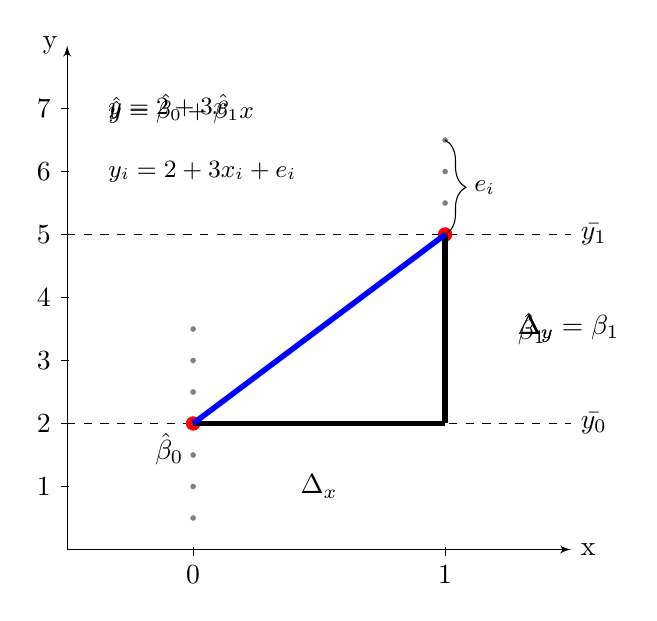
\begin{tikzpicture}[>=latex', scale=0.8]
        \draw[->] (0,0) node[below] (origin) {}  -- (8,0) node[right] (xaxis) {x};
        \draw[->] (origin) -- (0,8) node[left] (yaxis) {y};
        % x ticks
        \draw (2,1pt) -- (2,-3pt) node[anchor=north] {0};
        \draw (6,1pt) -- (6,-3pt) node[anchor=north] {1};
        % y ticks
        \foreach \y in {1,...,7}
             \draw (1pt,\y) -- (-3pt,\y) node[anchor=east] {$\y$};
        
        % points
        \foreach \y in {0.5,1.0,...,3.5} {
        	\draw[gray,fill] (2,\y) circle [radius=1pt];
        	\draw[gray,fill] (6,3+\y) circle [radius=1pt];
        }
        % y_0-bar
        \draw<2-4>[dashed] (0,2) -- (8,2) node[right] {$\bar{y_0}$};
        % y_1-bar
        \draw<2-4>[dashed] (0,5) -- (8,5) node[right] {$\bar{y_1}$};
        % mean points
        \draw<2->[red,fill] (2,2) circle [radius=3pt];
        \draw<2->[red,fill] (6,5) circle [radius=3pt];
        
        % slope
        \draw<3-4>[solid, line width=2pt] (2,2) -- (6,2);
        \draw<3-5>[solid, line width=2pt] (6,2) -- (6,5);
        \node<3-4>(deltax) at (4,1) {$\Delta_x$};
        \node<3>[right](deltay) at (7,3.5) {$\Delta_y$};
        \node<4>[right](deltay) at (7,3.5) {$\Delta_y = \beta_1$};
        \node<5>[right](deltay) at (7,3.5) {$\hat{\beta}_1$};
        
        \draw<4->[blue, solid, line width=2pt] (2,2) -- (6,5);
        \node<4-5>[below left](b0) at (2,2) {$\hat{\beta}_0$};
        
        \node<5>[right](eq) at (0.5,7) {\small $\hat{y} = \hat{\beta}_0 + \hat{\beta}_1 x$};
        \node<6->[right](eq) at (0.5,7) {\small $\hat{y} = 2 + 3 x$};
        \node<7->[right](eq) at (0.5,6) {\small $y_i = 2 + 3 x_i + e_i$};
        \draw<7->[right,decorate,decoration={brace,mirror,amplitude=7.5pt}] (6,5)  -- (6,6.5)
        	node [right, pos=0.5, xshift=7] {\small $e_i$};
    \end{tikzpicture}
    \end{center}
}

% OLS only makes sense in a linear world

\frame{
	\frametitle{Systematic versus unsystematic component of the data}
	\begin{itemize}\itemsep1em
    	\item Systematic: Regression line (slope)
    		\begin{itemize}
    		\item Linear regression estimates the conditional means of the population data (i.e., $E[Y|X]$)
    		\end{itemize}
    	\item Unsystematic: Error term is the deviation of observations from the line
    		\begin{itemize}
        		\item The difference between each value $y_i$ and $\hat{y}_i$ is the \textit{residual}: $e_i$
        		\item OLS produces an estimate of the relationship between X and Y that minimizes the \textit{residual sum of squares}
    		\end{itemize}
	\end{itemize}
}

\frame{
	\frametitle{Why are there residuals?}
	\begin{itemize}\itemsep1em
		\item<2-> Omitted variables
		\item<2-> Measurement error
		\item<2-> Fundamental randomness
	\end{itemize}
}

\againframe<2-3>{dummy}

\againframe<2-3>{ways}


\frame{
	\frametitle{Bivariate Regression II}
	\begin{itemize}\itemsep1em
	\item $Y$ is continuous
	\item $X$ is continuous (and randomized)
	\item How do we know if the treatment $X$ had an effect on $Y$?\\
		\begin{itemize}
		\item Correlation coefficient ($\rho$)
		\item Regression coefficient (slope; $\beta_1$)
		\end{itemize}
	\end{itemize}
}

\frame<1>[label=correlation]{
	\frametitle{Correlation Coefficient ($\rho$)}
	\begin{itemize}\itemsep1em
	\item Measures how well a scatterplot is represented by a straight (non-horizontal) line
	\item<2-> Formal definition: 
		$\frac{Cov(X,Y)}{\sigma_X \sigma_y}$
	\item<2-> As a reminder:\\
		\begin{itemize}\itemsep1em
		\item $Cov(x,y) = \sum_{i=1}^{n}(x_i - \bar{x})(y_i - \bar{y})$
		\item $s_x = \sqrt{\sum_{i=1}^{n}(x_i - \bar{x})^2}$
		\end{itemize}
	\end{itemize}
}

\frame{
	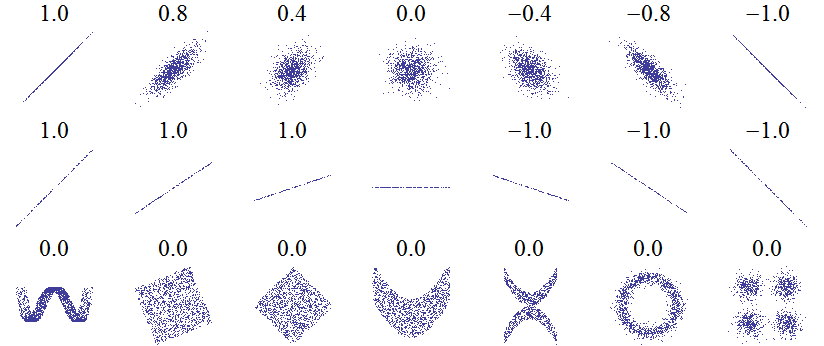
\includegraphics[width=\textwidth]{images/correlation}
}

\againframe<1->{correlation}

\frame{
	\frametitle{OLS Coefficient ($\beta_1$)\footnote{Multivariate formula involves matrices; Week 20}}
	\begin{itemize}\itemsep1em
	\item Measures $\Delta Y$ given $\Delta X$
	\item<2-> Formal definition: 
		$\frac{Cov(X,Y)}{Var(X)}$
	\item<2-> As a reminder:\\
		\begin{itemize}\itemsep1em
		\item $Cov(x,y) = \sum_{i=1}^{n}(x_i - \bar{x})(y_i - \bar{y})$
		\item $Var(x) = \sum_{i=1}^{n}(x_i - \bar{x})^2$
		\end{itemize}
	\item<3-> $\hat{\rho}$ and $\hat{\beta_1}$ are just scaled versions of $\widehat{Cov}(x,y)$
	\end{itemize}
}

\frame<1-6>[label=math]{
	\frametitle{Minimum Mathematical Requirements}
	\begin{enumerate}\itemsep1em
    	\item<1-> Do we need variation in $X$?
    		\begin{itemize}
        		\item<2-> Yes, otherwise dividing by zero
    		\end{itemize}
    	\item<3-> Do we need variation in $Y$?
    		\begin{itemize}
        		\item No, $\hat{\beta}_1$ can equal zero
    		\end{itemize}
    	\item<5-> How many observations do we need?
    		\begin{itemize}
    		\item<6-> $n \ge k$, where $k$ is number of parameters to be estimated
    		\end{itemize}
    	\item<7-> Can we have highly correlated regressors?
    		\begin{itemize}
    		\item<8-> Generally no (due to multicollinearity)
    		\end{itemize}
	\end{enumerate}
}

\frame<1-5>[label=scatter]{
	\begin{center}
	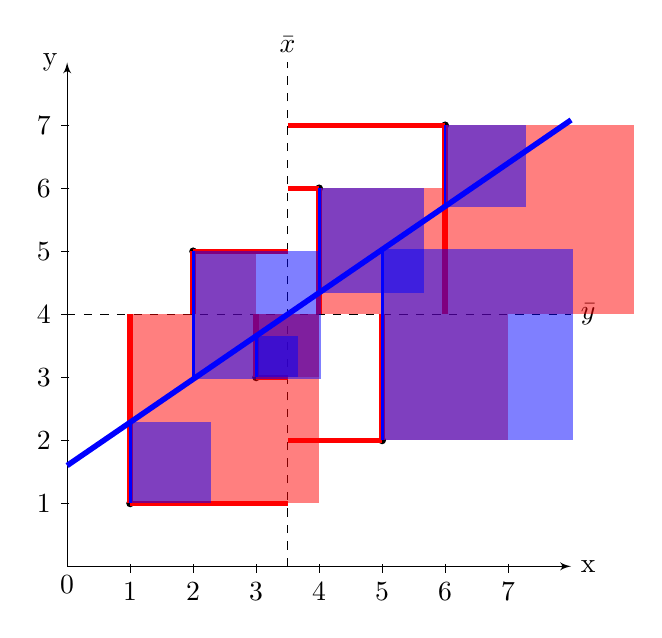
\begin{tikzpicture}[>=latex', scale=0.8]
        \draw[->] (0,0) node[below] (origin) {0}  -- (8,0) node[right] (xaxis) {x};
        \draw[->] (origin) -- (0,8) node[left] (yaxis) {y};
        % x ticks
        \foreach \x in {1,...,7}
        	\draw (\x,1pt) -- (\x,-3pt) node[anchor=north] {$\x$};
        % y ticks
        \foreach \y in {1,...,7}
             \draw (1pt,\y) -- (-3pt,\y) node[anchor=east] {$\y$};
        % points
        \draw[fill] (1,1) circle [radius=1.5pt];
        \draw[fill] (2,5) circle [radius=1.5pt];
        \draw[fill] (3,3) circle [radius=1.5pt];
        \draw[fill] (4,6) circle [radius=1.5pt];
        \draw[fill] (5,2) circle [radius=1.5pt];
        \draw[fill] (6,7) circle [radius=1.5pt];
        % x-bar
        \draw<2->[dashed] (3.5, 0) -- (3.5,8) node[above] {$\bar{x}$};
        % y-bar
        \draw<2->[dashed] (0,4) -- (8,4) node[right] {$\bar{y}$};
        
        % x-deviations
        \draw<3>[red, line width=2pt] (1,1) -- (3.5,1);
        \draw<3>[red, line width=2pt] (2,5) -- (3.5,5);
        \draw<3>[red, line width=2pt] (3,3) -- (3.5,3);
        \draw<3>[red, line width=2pt] (4,6) -- (3.5,6);
        \draw<3>[red, line width=2pt] (5,2) -- (3.5,2);
        \draw<3>[red, line width=2pt] (6,7) -- (3.5,7);
        % y-deviations
        \draw<4,6-7,10-11>[red, line width=2pt] (1,1) -- (1,4);
        \draw<4,6-7,10-11>[red, line width=2pt] (2,5) -- (2,4);
        \draw<4,6-7,10-11>[red, line width=2pt] (3,3) -- (3,4);
        \draw<4,6-7,10-11>[red, line width=2pt] (4,6) -- (4,4);
        \draw<4,6-7,10-11>[red, line width=2pt] (5,2) -- (5,4);
        \draw<4,6-7,10-11>[red, line width=2pt] (6,7) -- (6,4);
        
		\fill<7,11>[red, opacity=0.5] (1,1) rectangle (4,4);
		\fill<7,11>[red, opacity=0.5] (2,5) rectangle (3,4);
		\fill<7,11>[red, opacity=0.5] (3,3) rectangle (4,4);
		\fill<7,11>[red, opacity=0.5] (4,6) rectangle (6,4);
		\fill<7,11>[red, opacity=0.5] (5,2) rectangle (7,4);
		\fill<7,11>[red, opacity=0.5] (6,7) rectangle (9,4);

        % line
        \draw<5->[blue, line width=2pt] (0,1.6) -- (8,7.0856);
        
        % residuals
        \draw<8->[blue, line width=1pt] (1,1) -- (1,2.29);
        \draw<8->[blue, line width=1pt] (2,5) -- (2,2.97);
        \draw<8->[blue, line width=1pt] (3,3) -- (3,3.66);
        \draw<8->[blue, line width=1pt] (4,6) -- (4,4.34);
        \draw<8->[blue, line width=1pt] (5,2) -- (5,5.03);
        \draw<8->[blue, line width=1pt] (6,7) -- (6,5.71);
		
		\fill<9-11>[blue, opacity=0.5] (1,1) rectangle (2.29,2.29);
		\fill<9-11>[blue, opacity=0.5] (2,5) rectangle (4.03,2.97);
		\fill<9-11>[blue, opacity=0.5] (3,3) rectangle (3.66,3.66);
		\fill<9-11>[blue, opacity=0.5] (4,6) rectangle (5.66,4.34);
		\fill<9-11>[blue, opacity=0.5] (5,2) rectangle (8.03,5.03);
		\fill<9-11>[blue, opacity=0.5] (6,7) rectangle (7.29,5.71);

		
    \end{tikzpicture}
    \end{center}
}

\frame{
	\frametitle{Calculations}
	\begin{tabular}{rrrrrr} \hline
	$x_i$ & $y_i$ & $x_i - \bar{x}$ & $y_i - \bar{y}$ & $(x_i - \bar{x})(y_i - \bar{y})$ & $(x_i - \bar{x})^2$\\ \hline
	1 & 1 & ? & ? & ? & ? \\
	2 & 5 & ? & ? & ? & ? \\
	3 & 3 & ? & ? & ? & ? \\
	4 & 6 & ? & ? & ? & ? \\
	5 & 2 & ? & ? & ? & ? \\
	6 & 7 & ? & ? & ? & ? \\ \hline
	\end{tabular}
}
% mean(x) = 3.5
% mean(y) = 4
% cov(x,y) = 12
% var(x) = 17.5
% slope = 0.6857143

\frame{
	\frametitle{Intercept $\hat{\beta}_0$}
	\begin{itemize}\itemsep1em
	\item Simple formula: $\hat{\beta}_0 = \bar{y} - \hat{\beta}_1 \bar{x}$
	\item<2-> Intuition: OLS fit always runs through point $(\bar{x}, \bar{y})$
	\item<3-> Ex.: $\hat{\beta}_0 = 4 - 0.6857 * 3.5 = 1.6$
	\item<4-> $\hat{y} = 1.6 + 0.6857 \hat{x}$
	\end{itemize}
}

\againframe<5>{scatter}

% CEF: compare $\bar{Y}$ and $E[Y|X=x]$

\againframe<3-4>{ways}


\frame{
	\frametitle{OLS Minimizes SSR}
	\begin{itemize}\itemsep1em
    	\item Total Sum of Squares (SST): $\sum_{i=1}^{n}(y_i - \bar{y})^2$
    	\item We can partition SST into two parts (ANOVA):
    		\begin{itemize}
    		\item Explained Sum of Squares (SSE)
    		\item Residual Sum of Squares (SSR)
    		\end{itemize}
    	\item $SST = SSE + SSR$
    	\item OLS is the line with the lowest SSR
	\end{itemize}
}

\againframe<5-11>{scatter}

\frame{\frametitle{Questions about OLS calculations?}}


\frame[label=anygood]{
	\frametitle{Are Our Estimates Any Good?}
	Yes, if:\\
	\begin{enumerate}\itemsep1em
   		\item Works mathematically
   		\item Causally valid theory
   		\item Linear relationship between $X$ and $Y$
   		\item $X$ is measured without error
   		\item No missing data (or MCAR; see Lecture 5)
   		\item No confounding
	\end{enumerate}
}


\frame{
	\frametitle{Linear Relationship}
	\begin{itemize}\itemsep1em
    	\item If linear, no problems
    	\item If non-linear, we need to transform
    		\begin{itemize}
        		\item Power terms (e.g., $x^2$, $x^3$)
        		\item log (e.g., $log(x)$)
        		\item Other transformations
        		\item If categorical: convert to set of indicators
        		\item Multivariate interactions (next week)
    		\end{itemize}
	\end{itemize}
}

\frame{
	\frametitle{Coefficient Interpretation Activity}
	\begin{itemize}\itemsep1em
	\item Four types of variables:
		\begin{enumerate}
		\item Indicator (0,1)
		\item Categorical
		\item Ordinal
		\item Interval
		\end{enumerate}
	\item How do we interpret a coefficient on each of these types of variables?
	\end{itemize}
}

\frame{
	\frametitle{Notes on Interpretation}
	\begin{itemize}\itemsep1em
	\item<1-> Effect $\beta_1$ is constant across values of $x$
	\item<2-> That is not true when there are:
		\begin{itemize}
		\item Interaction terms (next week)
		\item Nonlinear transformations (e.g., $x^2$)
		\item Nonlinear regression models (e.g., logit/probit)
		\end{itemize}
	\item<3-> Interpretations are sample-level
		\begin{itemize}
		\item Sample representativeness determines generalizability
		\end{itemize}
	\item<4-> Remember uncertainty
		\begin{itemize}
		\item These are \textit{estimates}, not population parameters
		\end{itemize}
	\end{itemize}
}



\frame{
	\frametitle{Measurement Error in Regressor(s)}
	\begin{itemize}\itemsep1em
    	\item We want effect of $x$, but we observe $x^{*}$, where $x = x^{*} + w$:
    	\begin{align*}
    	y & = \beta_0 + \beta_1 x^{*} + \epsilon\\
    	 & = \beta_0 + \beta_1 (x - w) + \epsilon\\
    	 & = \beta_0 + \beta_1 x + (\epsilon - \beta_1 w)\\
    	 & = \beta_0 + \beta_1 x + v
    	\end{align*}
	\end{itemize}
}

\frame{
	\frametitle{Measurement Error in Regressor(s)}
	\begin{itemize}\itemsep1em
    	\item Produces \textit{attenuation}: as measurement error increases, $\beta_1 \rightarrow 0$
    	\item Our coefficients fit the observed data
    	\item But they are \textit{biased} estimates of our population equation
    		\begin{itemize}
    		\item This applies to all $\hat{\beta}$ in a multivariate regression
    		\item Direction of bias is unknown
    		\end{itemize}
	\end{itemize}
}


\frame{
	\frametitle{Measurement Error in $Y$}
	\begin{itemize}\itemsep1em
    	\item Not necessarily a problem
    	\item If \textit{random} (i.e., uncorrelated with $x$), it costs us precision
    	\item If \textit{systematic}, who knows?!
    	\item If \textit{censored}, see Lectures 11 and/or 12
	\end{itemize}
}


\frame{
	\frametitle{Missing Data}
	\begin{itemize}\itemsep1em
	\item Missing data can be a big problem
	\item We will discuss it in Lecture 5
	\end{itemize}
}

\frame{
	\frametitle{Confounding (Selection Bias)}
	\begin{itemize}\itemsep1em
	\item If $x$ is not randomly assigned, potential outcomes are not independent of $x$
	\item Other factors explain why a unit $i$ received their particular value $x_i$
	\vspace{1em}
	\item In matching, we obtain this \textit{conditional independence} by comparing units that are identical on all confounding variables
	\end{itemize}
}

\frame{
	\frametitle{Omitted Variables}
	{\small
	$\underbrace{E[Y_i| X_i = 1] - E[Y_i | X_i = 0] =}_{\text{Naive Effect}}$\\
	\vspace{1em}
	$\underbrace{E[Y_{1i}|X_i =1] - E[Y_{0i} | X_i = 1]}_{\text{Treatment Effect on Treated (ATT)}} + \underbrace{E[Y_{0i}|X_i = 1] - E[Y_{0i}|X_i=0]}_{\text{Selection Bias}}$
	}
	\vspace{1em}
}

\frame[label=causalgraph]{
	\begin{center}
	\begin{tikzpicture}[>=latex',circ/.style={draw, shape=circle, node distance=5cm, line width=1.5pt}]
        \draw[->] (0,0) node[left] (X) {X} -- (2.5,0) node[right] (D) {D};
        \draw[->] (3.1,0) -- (5,0) node[right] (Y) {Y};
        \draw[->] (-3,4) node[above] (Z) {Z} -- (X);
        \draw[->] (Z) -- (Y);
        \draw[->] (5,2) node[above] (A) {A} -- (Y);
        \draw[->] (-2,0) node[left] (B) {B} -- (X);
        \draw[->] (X) -- (2,-2) node[right] (C) {C};
    \end{tikzpicture}
    \end{center}
}

\frame{
	\frametitle{Omitted Variable Bias}
	\begin{itemize}
	\item We want to estimate:
	\begin{align*}
	Y = \beta_0 + \beta_1 X + \beta_2 Z + \epsilon
	\end{align*}
	\item We actually estimate:
	\begin{align*}
	\tilde{y} & = \tilde{\beta_0} + \tilde{\beta_1} x + \epsilon\\
	& = \tilde{\beta_0} + \tilde{\beta_1} x + (0 * z) + \epsilon\\
	& = \tilde{\beta_0} + \tilde{\beta_1} x + \nu
	\end{align*}
	\item Bias: $\tilde{\beta}_1 = \hat{\beta}_1 + \hat{\beta}_2 \tilde{\delta}_1$, where $\tilde{z} = \tilde{\delta}_0 + \tilde{\delta}_1 x$
	\end{itemize}
}

\frame{
	\frametitle{Size and Direction of Bias}
	\begin{itemize}
	\item Bias: $\tilde{\beta}_1 = \hat{\beta}_1 + \hat{\beta}_2 \tilde{\delta}_1$, where $\tilde{z} = \tilde{\delta}_0 + \tilde{\delta}_1 x$
	\end{itemize}
	\vspace{1em}
	\begin{center}
	\begin{tabular}{lll}
		              & $Corr(x,z)<0$ & $Corr(x,z)>0$ \\ \hline
		$\beta_2 < 0$ & Positive      & Negative      \\
		$\beta_2 > 0$ & Negative      & Positive      \\ \hline
	\end{tabular}
	\end{center}
}


\frame{
	\frametitle{Aside: Three Meanings of ``Endogeneity''}
	Formally endogeneity is when $Cov(X,\epsilon) \neq 0$
	\vspace{1em}
	\begin{enumerate}\itemsep1em
	\item Measurement error in regressors
	\item Omitted variables associated with included regressors 
		\begin{itemize}
		\item ``Specification error''
		\item Confounding
		\end{itemize}
	\item Lack of temporal precedence
	\end{enumerate}
}


\frame{
	\frametitle{Example: Englebert}
	\begin{itemize}\itemsep2em
	\item What is his research question?
	\item What is his theory? What does the graph look like?
	\item What is his analysis?
	\end{itemize}
}


\frame{
	\frametitle{Common Conditioning Strategies}
	\begin{enumerate}\itemsep1em
    	\item<2-> Condition on nothing (``naive effect'')
    	\item<3-> Condition on some variables
    	\item<4-> Condition on all observables
	\end{enumerate}
	\vspace{1em}
	\onslide<5->{Which of these are good strategies?}
}


\frame<1-2>[label=what]{
	\frametitle{What goes in our regression?}
	\begin{itemize}\itemsep1em
    	\item Use theory to build causal models
    		\begin{itemize}
    		\item Often, a causal graph helps
    		\end{itemize}
    	\item Some guidance:
    		\begin{itemize}
    		\item<2-> Include confounding variables
	    	\item<3-> Do not include post-treatment variables
	    	\item<4-> Do not include \textit{colinear} variables
    		\item<5-> Including irrelevant variables costs certainty
    		\item<6-> Including variables that affect $Y$ alone increases certainty
    		\end{itemize}
	\end{itemize}
}

\againframe{causalgraph}

\againframe<2-3>{what}

\againframe{causalgraph}

\frame{
	\frametitle{Post-treatment Bias}
	\begin{itemize}\itemsep1em
	\item We usually want to know the \textbf{total effect} of a cause
	\item If we include a mediator, $D$, of the $X \rightarrow Y$ relationship, the coefficient on $X$:
		\begin{itemize}
    		\item Only reflects the \textbf{direct} effect
    		\item Excludes the \textbf{indirect} effect of $X$ through $M$
		\end{itemize}
	\item So don't control for mediators!
	\end{itemize}
}

\againframe<3-4>{what}

\againframe<6-8>{math}

\againframe<4-6>{what}

\againframe{causalgraph}

\frame{\frametitle{Questions about specification?}}

\frame{
	\frametitle{Multivariate Regression Interpretation}
	\begin{itemize}\itemsep1em
	\item All our interpretation rules from earlier still apply in a multivariate regression
	\item Now we interpret a coefficient as an effect ``all else constant''
	\item Generally, not good to give all coefficients a causal interpretation
		\begin{itemize}
		\item Think ``forward causal inference''
		\item We're interested in the $X \rightarrow Y$ effect
		\item All other coefficients are there as ``controls''
		\end{itemize}
	\end{itemize}
}

\frame{
	\frametitle{From Line to Surface I}
	\begin{itemize}\itemsep1em
	\item In simple regression, we estimate a \textbf{line}
	\item In multiple regression, we estimate a \textbf{surface}
	\item Each coefficient is the \textit{marginal effect}, all else constant (at mean)
	\item This can be hard to picture in your mind
	\end{itemize}
}

\frame{
	\frametitle{From Line to Surface II}
	\begin{center}
	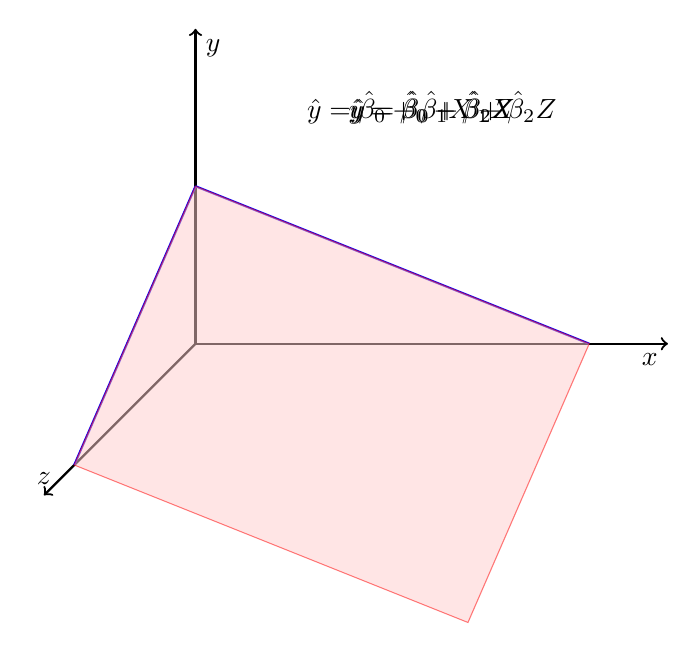
\begin{tikzpicture}
	    \draw[thick,->] (0,0,0) -- (6,0,0) node[anchor=north east]{$x$};
	    \draw[thick,->] (0,0,0) -- (0,4,0) node[anchor=north west]{$y$};
	    \draw<1> (3,3,0) node {$\hat{y} = \hat{\beta}_0 + \hat{\beta}_1 X$};
        \draw<2> (3,3,0) node {$\hat{y} = \hat{\beta}_0 + \hat{\beta}_2 Z$};
	    \draw<3> (3,3,0) node {$\hat{y} = \hat{\beta}_0 + \hat{\beta}_1 X + \hat{\beta}_2 Z$};
	    \draw<1,3>[thick, blue] (0,2,0) -- (5,0,0);
	    \draw<2->[thick,->] (0,0,0) -- (0,0,5) node[anchor=south]{$z$};
	    \draw<2->[thick, blue] (0,2,0) -- (0,0,4);
	    \filldraw<3->[draw=red,fill=red!20,opacity=0.5]
	        (0,2,0) -- (0,0,4) -- (5,-2,4) -- (5,0,0) -- cycle;
	\end{tikzpicture}
	\end{center}
}


\againframe{anygood}

\frame{
	\frametitle{OLS is BLUE}
	\begin{itemize}\itemsep1em
	\item BLUE: Best Linear Unbiased Estimator
	\item Gauss Markov Assumptions:
		\begin{enumerate}
		\item Linearity in parameters
		\item Random sampling
		\item No multicollinearity
		\item Exogeneity ($E[\epsilon|\mathbf{X}] = 0$)
		\item Homoskedasticity ($Var(\epsilon|\mathbf{X}) = \sigma^2$)
		\end{enumerate}
	\item Assumptions 1--4 prove OLS is unbiased
	\item Assumption 5 proves OLS is the \textit{best} estimator
	\end{itemize}
}



\frame{
	\frametitle{Squared vs. Absolute Errors}
	\begin{itemize}\itemsep1em
	\item Conventionally use Sum of Squared Errors
	\item Using absolute errors is also unbiased
	\item Sum of Squared Errors:
		\begin{itemize}
		\item more heavily weights outliers
		\item has a smaller variance
		\end{itemize} 
	\item Thus OLS is \textbf{B}est\textbf{LUE}
	\end{itemize}
}







\section{Goodness-of-Fit}
\frame{\tableofcontents[currentsection]}

\frame{
	\frametitle{Goodness-of-Fit}
	\begin{itemize}\itemsep1em
	\item We want to know: ``How good is our model?''
	\item<2-> We can answer:\\
		``How well does our model fit the observed data?''
	\item<3-> Is this what we want to know?
	\end{itemize}
}

\frame{
	\frametitle{Correlation}
	\begin{itemize}\itemsep1em
	\item Definition: $Corr(x,y) = \hat{r}_{x,y} = \frac{Cov(x,y)}{(n-1) s_x s_y}$
	\item Slope $\hat{\beta}_1$ and correlation $\hat{r}_{x,y}$ are simply different scalings of $Cov(x,y)$
	\item Interpretation: How well the bivariate relationship is summarized by a cloud of points?
	\item Units: none (range -1 to 1)
	\end{itemize}
}

\frame{
	\frametitle{Coefficient of Determination ($R^2$)}
	\begin{itemize}\itemsep1em
	\item Definition: $R^2 = \hat{r}_{x,y}^2 = \frac{SSE}{SST} = 1 - \frac{SSR}{SST}$
	\item Interpretation: How much of the total variation in $y$ is explained by the model?
	\item But, $R^2$ increases simply by adding more variables
	\item So, Adjusted-$R^2 = R^2 - (1 - R^2)\frac{k}{n-k-1}$, where $k$ is number of regressors
	\item Units: none (range 0 to 1)
	\end{itemize}
}

\frame{
	\frametitle{Standard Error of the Regression (SER)}
	\begin{itemize}\itemsep1em
	\item ``Root mean squared error'' or just $\sigma$
	\item Definition: $\hat{\sigma} = \sqrt{\frac{SSR}{n-p}}$, where $p$ is number of parameters estimated
	\item Interpretation: How far, on average, are the observed $y$ values from their corresponding fitted values $\hat{y}$
		\begin{itemize}
		\item $sd(y)$ is how far, on average, a given $y_i$ is from $\bar{y}$
		\item $\sigma$ is how far, on average, a given $y_i$ is from $\hat{y}_i$
		\end{itemize}
	\item Units: same as $y$ (range 0 to $sd(y)$)
	\end{itemize}
}

\frame{
	\frametitle{The F-test}
	\begin{itemize}\itemsep1em
	\item Definition: Test of whether any of our coefficients differ from zero
		\begin{itemize}
		\item In a bivariate regression, $F=t^2$
		\end{itemize}
	\item Interpretation: Do any of the coefficients differ from zero?
		\begin{itemize}
		\item Not a very interesting measure
		\end{itemize}
	\item Units: none (range 0 to $\infty$)
	\end{itemize}
}

\begin{frame}[fragile,label=statareg]
\scriptsize
\begin{columns}
    \column{\dimexpr\paperwidth-20pt}
\begin{verbatim}
. reg growth lcon

      Source |       SS       df       MS              Number of obs =      44
-------------+------------------------------           F(  1,    42) =    0.09
       Model |  .000038348     1  .000038348           Prob > F      =  0.7615
    Residual |  .017255198    42  .000410838           R-squared     =  0.0022
-------------+------------------------------           Adj R-squared = -0.0215
       Total |  .017293546    43  .000402175           Root MSE      =  .02027

------------------------------------------------------------------------------
      growth |      Coef.   Std. Err.      t    P>|t|     [95% Conf. Interval]
-------------+----------------------------------------------------------------
        lcon |  -.0017819   .0058325    -0.31   0.761    -.0135524    .0099886
       _cons |   .0158988   .0390155     0.41   0.686    -.0628376    .0946353
------------------------------------------------------------------------------

\end{verbatim}
    
\end{columns}
\end{frame}





\section{Analysis of Complex Surveys}
\frame{\tableofcontents[currentsection]}

\frame{\frametitle{}}


\section{Panel Studies and Regression}
\frame{\tableofcontents[currentsection]}

\frame{\frametitle{}}



\appendix
\frame{}

\end{document}
